\documentclass[11pt]{article}

\usepackage{amsmath}
\usepackage{amssymb}
\usepackage{array}
\usepackage{geometry}
\usepackage{enumitem}
\usepackage{float}
\usepackage{cancel}
\usepackage{graphicx}
\usepackage[labelformat=empty]{caption}
\usepackage{booktabs}
\usepackage{xcolor}

\geometry{
	a4paper,
 	left=20mm,
 	top=20mm,
 	bottom=20mm,
}

\setlength{\parindent}{0pt}

\begin{document}

\section{Allgemein}

\subsection{Trigonometrie}

\begin{center}
	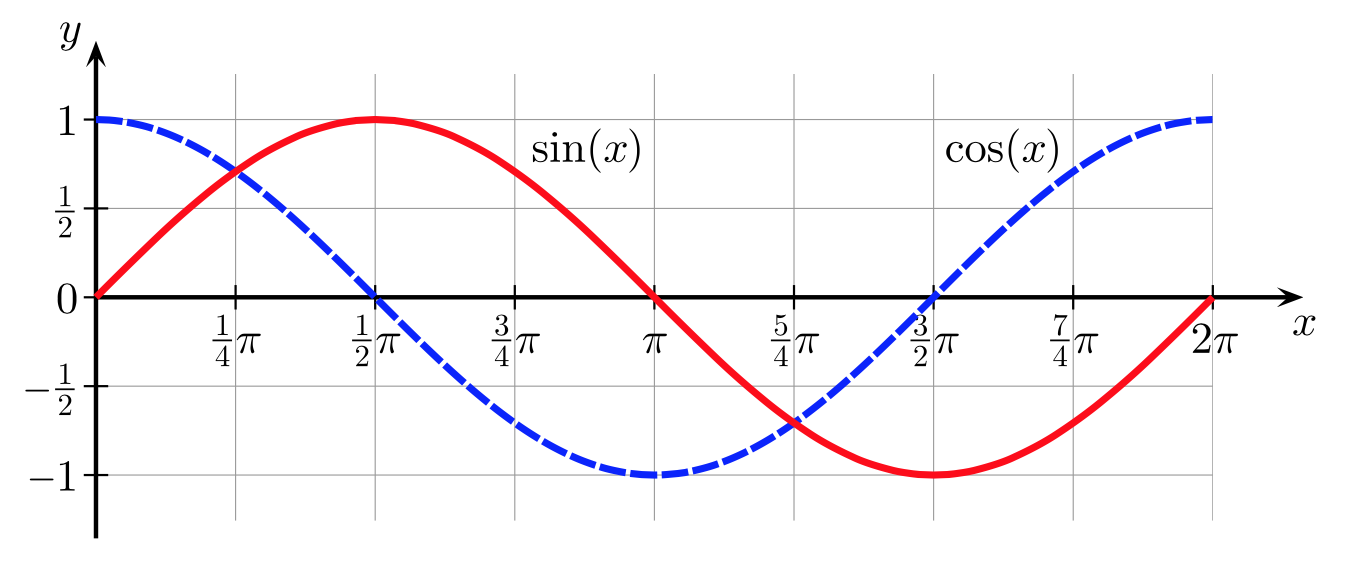
\includegraphics[width=\linewidth,keepaspectratio=true]{images/trigonometry}
\end{center}

\begin{center}
	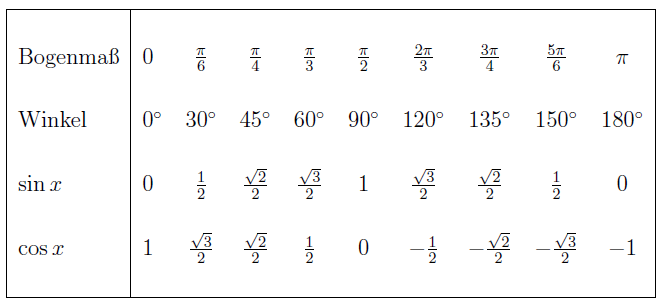
\includegraphics[width=300pt]{images/trigonometry_table}
\end{center}

\begin{equation*}
\begin{split}
	\tan(x) & = \frac{\sin(x)}{\cos(x)} \\
	\sin(2x) & = 2\sin(x)\cos(x) \\
	\sin(\alpha + \beta) & = \sin(\alpha)\cos(\beta) + \cos(\alpha)\sin(\beta) \\
	\cos(\alpha + \beta) & = \cos(\alpha)\cos(\beta) + \sin(\alpha)\sin(\beta) \\
	\cos^2(x) & = \frac{1 + \cos(2x)}{2} \\
	\sin^2(x) + \cos^2(x) & = 1
\end{split}
\end{equation*}

\begin{minipage}[c]{0.5\textwidth}
\subsection{Potenzgesetze}

\begin{equation*}
\begin{split}
	a^0 & = 1 \\
	a^1 & = a \\
	a^m \cdot a^n & = a^{m+n} \\
	(a^n)^m & = a^{nm} \\
	\frac{a^n}{a^m} & = a^{n-m} \\
	a^{-n} & = \frac{1}{a^n} \\
	a^{\frac{b}{n}} & = \sqrt[n]	{a^b} \\
\end{split}
\end{equation*}
\end{minipage}
%
\begin{minipage}[c]{0.5\textwidth}
\subsection{Logarithmus}

\begin{equation*}
\begin{split}
	\log(0) & = \text{undef.} \\
	\log(1) & = 0 \\
	x \log_a(y) & \Leftrightarrow a^x = y \\
	- \log(x) & = \log(\frac{1}{x}) \\
	\log(x) - \log(y) & = \log(\frac{x}{y}) \\
	\frac{\log(x)}{\log(a)} & = \log_a(x)
\end{split}
\end{equation*}
\end{minipage}

\section{Integration}

\subsection{Elementare Integrale}

\begin{table}[H]
\centering
\begin{tabular}{|c|c|c|}
\hline
$f'(x)$ & $f(x)$ & $F(x)$ \\ \specialrule{.1em}{0em}{0em} 
$\frac{f'(x)g(x) - f(x)g'(x)}{g(x)^2}$ & $\frac{f(x)}{g(x)}$ &  \\ \hline
$0$ & $c$ & $cx$ \\ \hline
$r\cdot x^{r-1}$ & $x^r$ & $\frac{x^{r+1}}{r+1}$ \\ \hline
$-\frac{1}{x^2} = -x^{-2}$ & $\frac{1}{x} = x^{-1}$ & $\ln|x|$ \\ \hline
$\frac{1}{2\sqrt{x}} = \frac{1}{2}x^{-\frac{1}{2}}$ & $\sqrt{x} = x^{\frac{1}{2}}$ & $\frac{2}{3}x^\frac{3}{2}$ \\ \hline
$\cos(x)$ & $\sin(x)$ & $-\cos(x)$ \\ \hline
$-\sin(x)$ & $\cos(x)$ & $\sin(x)$ \\ \hline
$1 + \tan^2(x) = \frac{1}{\cos^2(x)}$ & $\tan(x)$ & $-\ln|\cos(x)|$ \\ \hline
$e^x$ & $e^x$ & $e^x$ \\ \hline
$c\cdot e^{cx}$ & $e^{cx}$ & $\frac{1}{c}\cdot e^{cx}$ \\ \hline
$\ln(c)\cdot c^x$ & $c^x$ & $\frac{c^x}{\ln(c)}$ \\ \hline
$\frac{1}{x}$ & $\ln|x|$ & $x(\ln|x| - 1)$ \\ \hline
$\frac{1}{\ln(a) \cdot x}$ & $\log_a|x|$ & $\frac{x}{\ln(a)}(\ln|x| -1)$ \\ \hline
$\frac{1}{\sqrt{1-x^2}}$ & $\arcsin(x)$ & $x\cdot\arcsin(x) + \sqrt{1-x^2}$ \\ \hline
$-\frac{1}{\sqrt{1-x^2}}$ & $\arccos(x)$ & $x\cdot\arccos(x) - \sqrt{1-x^2}$ \\ \hline
$\frac{1}{1+x^2}$ & $\arctan(x)$ & $x\cdot \arctan(x) - \frac{1}{2}\ln(1+x^2)$ \\ \hline
$\cosh(x)$ & $\sinh(x) = \frac{e^x - e^{-x}}{2}$ & $\cosh(x)$ \\ \hline
$\sinh(x)$ & $\cosh(x) = \frac{e^x + e^{-x}}{2}$ & $\sinh(x)$ \\ \hline
$\frac{1}{\cosh^2(x)}$ & $\tanh(x)$ & $\log(\cosh(x))$ \\ \hline
\end{tabular}
\end{table}

\subsection{Regeln}

\begin{equation*}
\begin{split}
	\textbf{Direkter Integral}\quad & \int f(g(x))g'(x)\ dx = F(g(x)) \\
	\textbf{Partielle Integration}\quad & \int f' \cdot g\ dx = f \cdot g - \int f \cdot g'\ dx \\
	\textbf{mit Polynomen}\quad & \int\frac{p(x)}{q(x)}\ dx \Rightarrow\ \text{Partialbruchzerlegung} \\
	\textbf{Substitution}\quad & \int_a^b f(\varphi(t))\varphi'(t)\ dt = \int_{\varphi(a)}^{\varphi(b)} f(x)\ dx\ \text{mit}\ x = \varphi(t)
\end{split}
\end{equation*}

\subsection{Tipps}

\begin{equation*}
\begin{split}
	\int\tan x\ dx & = \int\frac{\sin x}{\cos x}\ dx = -\log|\cos(x)| \\
	\int \frac{1}{x - \alpha}\ dx & = \log(x-\alpha) \\
	\int\frac{\frac{1}{\alpha}}{1+(\frac{x}{\alpha})^2}\ dx & = \arctan(x) \\
	\int \sin^2(x)\ dx & = \frac{1}{2}(x - \sin(x)\cos(x)) + C \\
	\int \cos^2(x)\ dx & = \frac{1}{2}(x + \sin(x)\cos(x)) + C \\
	\int \sqrt{x^2+1}\ dx & = \sinh(x) + C
\end{split}
\end{equation*}

\section{Vektorfelder}

\subsection{Differenzial (f{\"u}r f: $\mathbb{R}^n \mapsto \mathbb{R}^m$)}

\begin{equation*}
	df = \begin{pmatrix}
		\frac{\partial f_1}{\partial x_1} & ... & \frac{\partial f_1}{\partial x_n} \\
		... & ... & ... \\
		\frac{\partial f_m}{\partial x_1} & ... & \frac{\partial f_m}{\partial x_n}
	\end{pmatrix}
\end{equation*}

\subsection{Gradient (f{\"u}r f: $\mathbb{R}^n \mapsto \mathbb{R}$)}

\begin{equation*}
	\text{grad}(f)=\nabla f=
	\begin{pmatrix}
		\frac{\partial f}{\partial x_1}\\
		...\\
		\frac{\partial f}{\partial x_n}\\
	\end{pmatrix}
\end{equation*}

Der Gradient zeigt in die Richtung der maximalen Zuwachsrate von $f$ und seine L{\"a}nge ist gleich der maximalen {\"A}nderung von $f$.

\subsection{Hessematrix (f{\"u}r f: $\mathbb{R}^n \mapsto \mathbb{R}$)}

\begin{equation*}
	\text{Hess}(f)=
	\begin{pmatrix}
		\frac{\partial^2 f}{\partial^2x_1^2} & ... & \frac{\partial^2 f}{\partial x_1 \partial x_n}\\
		...&...&...\\
		\frac{\partial^2 f}{\partial x_n \partial x_1} & ... & \frac{\partial^2 f}{\partial x_n^2}
	\end{pmatrix}
\end{equation*}

\subsection{Rotation (f{\"u}r f: $\mathbb{R}^3 \mapsto \mathbb{R}^3$ oder f: $\mathbb{R}^2 \mapsto \mathbb{R}^2$)}

\begin{equation*}
	\text{In}\ \mathbb{R}^3:\ \text{rot}(\vec{v})=\nabla\times \vec{v} =
	\begin{pmatrix}
		\frac{\partial v_3}{\partial y} - \frac{\partial v_2}{\partial z}\\
		\frac{\partial v_1}{\partial z} - \frac{\partial v_3}{\partial x}\\
		\frac{\partial v_2}{\partial x} - \frac{\partial v_1}{\partial y}
	\end{pmatrix},\ \text{in}\ \mathbb{R}^2:\ \text{rot}(\vec{v}) = \frac{\partial v_2}{\partial x} - \frac{\partial v_1}{\partial y}
\end{equation*}

\emph{Bemerkung:} Falls $\text{rot}(\vec{v})=0$, dann ist $\vec{v}$ konservativ (Potenzialfeld).

\subsection{Divergenz (f{\"u}r f: $\mathbb{R}^n \mapsto \mathbb{R}^n$)}
\begin{equation*}
	\text{div}(v)= \frac{\partial v_1}{\partial x} + \frac{\partial v_2}{\partial y} + ... 
\end{equation*}

\subsection{Potenzialfeld}

Ein Potenzialfeld ist konservativ. Das Potenzial $\Phi$ eines Potenzialfeldes ist gleich:

\begin{equation*}
	\nabla \Phi = \vec{v}
\end{equation*}

F{\"u}r ein Potenzialfeld gilt $\text{rot}(\vec{v})=0$ und es erf{\"u}llt die \textbf{Integrabilit{\"a}tsbedinungen}:

\begin{equation*}
	\frac{\partial v_i}{\partial x_j}=\frac{\partial v_j}{\partial x_i},\forall i \neq j
\end{equation*}

\subsubsection*{Berechnung eines Potenzials}

\begin{equation*}
\begin{split}
	\text{gegeben:} \quad & \vec{v} = \begin{pmatrix}
		e^{xy}(1+xy) \\ e^{xy}x^2
	\end{pmatrix} \\
	\textbf{Nach y integrieren:} \quad & \frac{\partial\Phi}{\partial y} = e^{xy}x^2 \Rightarrow \Phi = \int e^{xy}x^2\ dy = xe^{xy} + C(x) \\
	\textbf{Nach x ableiten:} \quad & \frac{\partial\Phi}{\partial x} = e^{xy} + xye^{xy} + C' \stackrel{!}{=} e^{xy} + xye^{xy} \Rightarrow C' = 0 \Rightarrow C = \text{konst.} \\
	\textbf{Potenzial:} \quad & \Phi = xe^{xy} + \text{konst.}
\end{split}
\end{equation*}

\subsection{Koordinatentransformationen}

\subsubsection{Polarkoordinaten ($\mathbb{R}^2$)}

\begin{equation*}
	\textbf{Variablen:}\quad \begin{matrix}
		x = r\cos(\phi) \\ y = r\sin(\phi)
	\end{matrix} \quad \textbf{Volumenelement:}\quad \iint dxdy = \int_0^{2\pi} d\phi \int_0^R \boldmath{\textcolor{red}{r}}\ dr
\end{equation*}

\subsubsection{Elliptische Koordinaten ($\mathbb{R}^2$)}

\begin{equation*}
	\textbf{Variablen:}\quad \begin{matrix}
		x = ra\cos(\phi) \\ y = rb\sin(\phi)
	\end{matrix} \quad \textbf{Volumenelement:}\quad \iint dxdy = \boldmath{\textcolor{red}{ab}} \int_0^{2\pi} d\phi \int_0^R \boldmath{\textcolor{red}{r}} dr
\end{equation*}

\subsubsection{Zylinderkoordinaten ($\mathbb{R}^3$)}

\begin{equation*}
	\textbf{Variablen:}\quad \begin{matrix}
		x = r\cos(\phi) \\ y = r\sin(\phi) \\ z = z
	\end{matrix} \quad \textbf{Volumenelement:}\quad \iiint dxdydz = \int_{-Z}^{Z} dz \int_0^{2\pi} d\phi \int_0^R \boldmath{\textcolor{red}{r}}\ dr
\end{equation*}

\subsubsection{Kugelkoordinaten ($\mathbb{R}^3$)}

\begin{minipage}[c]{0.3\textwidth}
\centering
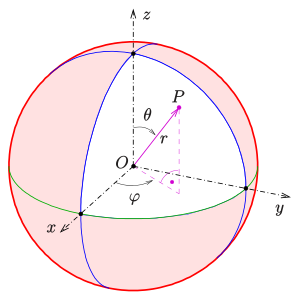
\includegraphics[width=\textwidth]{images/kugelkoordinaten}
\end{minipage}
%
\begin{minipage}[c]{0.7\textwidth}
\begin{equation*}
\begin{split}
	\textbf{Variablen:}\quad & \begin{matrix}
		x = r\sin(\theta)\cos(\varphi) \\ y = r\sin(\theta)\sin(\varphi) \\ z = r\cos(\theta)
	\end{matrix} \\
	\textbf{Volumenelement:} \quad & \iiint dxdydz = \int_0^{2\pi} d\varphi \int_0^\pi \boldmath{\textcolor{red}{\sin(\theta)}}\ d\theta \int_0^R \boldmath{\textcolor{red}{r^2}}\ dr\
\end{split}
\end{equation*}
\end{minipage}
	
\end{document}
